\documentclass[a4paper,12pt]{article}
\usepackage[left=2cm, right=2cm, top=2cm]{geometry}
\usepackage{graphicx} 
\usepackage[export]{adjustbox}
\usepackage{titlepic}
\usepackage{amssymb}
\usepackage{titling}
\usepackage[utf8]{inputenc}
\usepackage{listings}
\usepackage{color}
\usepackage[T1]{fontenc}
\usepackage[utf8]{inputenc}
\usepackage{wrapfig}
\usepackage{helvet}
\usepackage{fourier} 
\usepackage{array}
\usepackage{makecell}
%\usepackage[square,sort,comma,numbers]{natbib}
\usepackage{ragged2e}
\usepackage{placeins}
\bibliographystyle{IEEEtran}
\usepackage{float}
\setlength{\belowcaptionskip}{-15pt}
\renewcommand{\familydefault}{\sfdefault}
\newcommand{\squeezeup}{\vspace{-2.5mm}}
\definecolor{codegreen}{rgb}{0,0.6,0}
\definecolor{codegray}{rgb}{0.5,0.5,0.5}
\definecolor{codepurple}{rgb}{0.58,0,0.82}
\definecolor{backcolour}{rgb}{0.95,0.95,0.92}

\renewcommand\theadalign{bc}
\renewcommand\theadfont{\bfseries}
\renewcommand\theadgape{\Gape[4pt]}
\renewcommand\cellgape{\Gape[4pt]}

\usepackage{fancyhdr,lipsum}
\pagestyle{fancy}
\fancyhf{}% Clear header/footer

\usepackage{hyperref}
\hypersetup{
    colorlinks,
    %citecolor=gray,
    citecolor=black,
    filecolor=black,
    linkcolor=black,
    urlcolor=black,
    linktoc=all
}

\lstdefinestyle{mystyle}{
    backgroundcolor=\color{backcolour},   
    commentstyle=\color{codegreen},
    keywordstyle=\color{blue},
    numberstyle=\tiny\color{codegray},
    stringstyle=\color{codepurple},
    basicstyle=\tiny,
    breakatwhitespace=false,         
    breaklines=true,                 
    captionpos=b,                    
    keepspaces=true,                 
    numbers=left,                    
    numbersep=5pt,                  
    showspaces=false,                
    showstringspaces=false,
    showtabs=false,                  
    tabsize=2
}


\chead{%
  \ifcase\value{page}
  % empty test for page = 0
  \or % page=1
  \or % page = 2
  \or Haider Shafiq% page = 3
  \or Alexander Bolton% page = 4
  \or Alexander Bolton% page = 5
  \or Alexander Bolton% page = 6
  \or Alexander Bolton% page = 7
  \or Insert Author% page = 8
  \or Insert Author% page = 9
  \or Insert Author% page = 10
  \or Insert Author% page = 11
  \or Insert Author% page = 12
  \or Insert Author% page = 13
  \or Insert Author% page = 14
  \else
  % Empty chead here!
  \fi
}



\lstset{style=mystyle}

\pretitle{%
  \begin{center}
  \LARGE
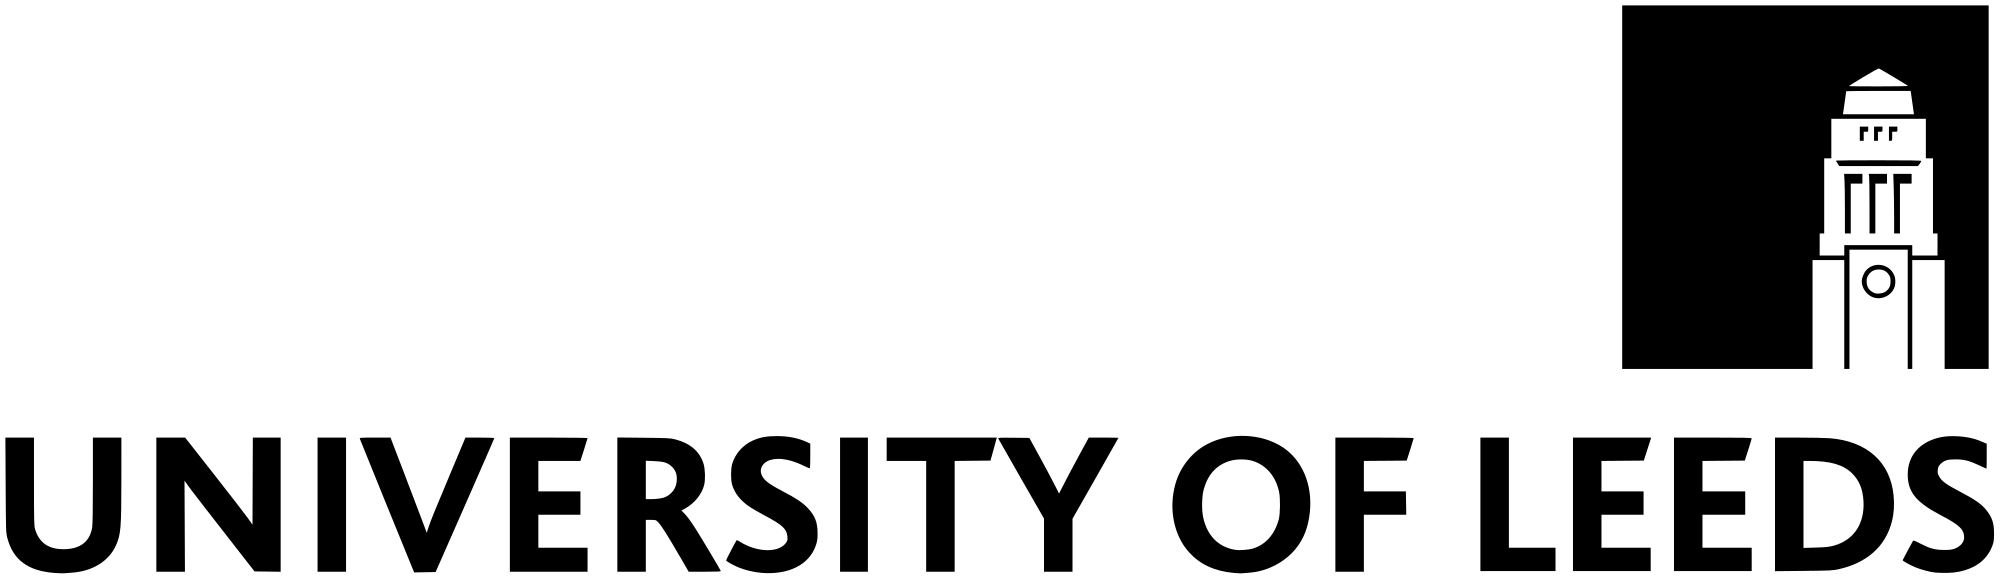
\includegraphics[width=0.5\textwidth, right]{UniLogo.png}\\[\bigskipamount]

\hspace{15cm}

\hspace{27cm}

\hspace{27cm}

\hspace{10cm}
}
\posttitle{\end{center}}	

\begin{document}

\title{\\ \textbf{ELEC5566M \\ Mini Project \\ \- \\ DE1-SoC Oscilloscope }}
\author{Alexander Bolton - 200938078 \\ Haider Shafiq - 201207577}
\date{May 2019}
\maketitle
\begin{center}
Submitted in accordance with the requirements for the degree of \\
Master of Science in Embedded Systems Engineering
\end{center}
\vfill
\begin{center}
The University of Leeds \\  School of Electronic and Electrical Engineering
\end{center}
\newpage

\tableofcontents
\newpage 
\section{Introduction}
\begin{flushleft}
This report shall discuss the group project for the FGPA Design for System-on-Chip module. The group consisted of Alexander Bolton, and Haider Shafiq. The project chosen was to design and develop a multi-channel oscilloscope on the DE1-SoC. The aim of this project was to take multiple input signals from a signal generator, and display them accurately on a separate monitor, via the VGA port of the DE1-SoC. \\ \- \\
The report shall cover the various parts of this project, and how they were then tested, as well as why they were needed. In chapter 2 the design of the VGA driver will be discussed, as well as the challenges presented with its development. The VGA port was used to output the waves to a separate monitor such that they can then be analysed.
Chapter 3 shall discuss the development of the ADC module. The ADC used was the one on-board the DE1-SoC. This ADC has 10 pins, a ground pin a voltage pin, and 8 pins which can act as separate channels. The data from the ADC shall be displayed on the VGA, and they will be waves will be seen on the monitor. Multiples signals will be given to the ADC via a signal generator, and the waves will be displayed on a separate monitor, via the VGA. \\ \- \\
In chapter 4 the design of the seven-segment display will be discussed. The seven-segment display will provide the user with the information of the waves on the screen, such as the voltage of the wave. This will be measured by the cursors on the screen which will be discussed in chapter 5. The controls for the system including two cursors in the x-axis and two cursors in the y-axis. These cursors will be controlled by the keys on the DE1-SoC board, and which cursor is being moved at which time shall be controlled by the switches on the board. The controls shall also acts as enable switches displaying, whether the cursors are being controlled, or whether the waves on screen are. The controls chapter will also discuss the design of the slower clock module, and the purpose of it.   \\ \- \\
Chapter 6 will discuss the design of the measurement's module.  The measurements module was the module responsible for calculating the wave information such as the voltage of each wave. This information was then displayed on the seven-segment display. Chapter 7 will discuss any problems encountered while completing this project, such as problems with the LT24 LCD, or problems with the Terasic ADDA ADC board. \\ \- \\
This report shall conclude in chapter 8 with an analysis of the overall work completed in the project, as well as any further work which could be undertaken as part of this project. This further work could be in the from of an expansion to the current work already completed, or any modifications to the current project which could improve it.  All the code will be put in the appendices at the end of this report, including the code for any test benches. 
\end{flushleft}
\newpage
\section{VGA}
\begin{flushleft}
For this project it was decided to make the wave as visible as possible it would be the most beneficial to use the Video Graphics Array (VGA) connector to connect the FPGA to a monitor. The VGA comprises of 3 buses of 8 bits for colour (Red, Green, Blue), a clock signal, a horizontal sync signal (HSync), and finally a vertical sync signal (VSync) as shown in Figure 1. The resolution chosen was 800x600 at a frequency of 75Hz. To carry out his resolution is required a clock of 49MHz (50MHz clock was used direct from the FPGA). All the timing specifications were found in the DE1-SoC manual (See Appendix A).\\
\begin{figure}[H]
	\centering
	\fbox{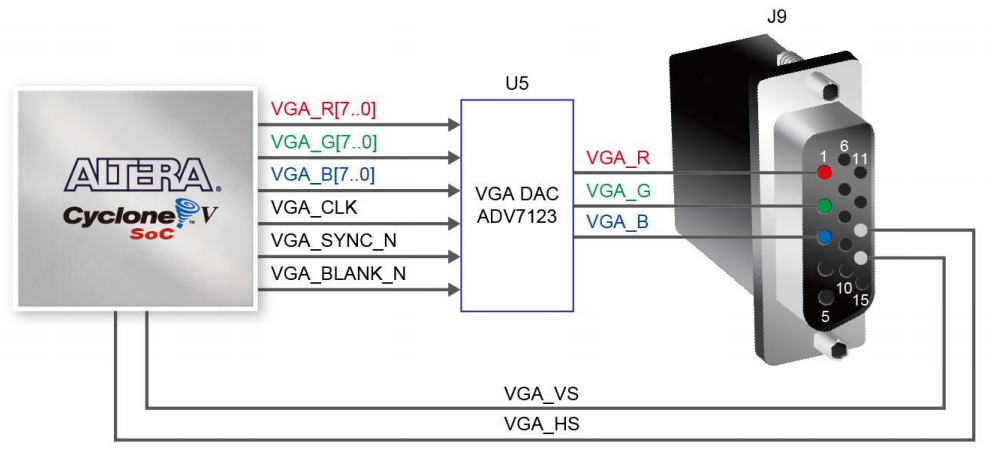
\includegraphics[width=0.5\textwidth]{./images/VGA.png}}
	\caption{VGA Pins \cite{terasic_2014}}
\end{figure}
The VGA signal is made up of 4 parts which are the Sync Signal, Back porch, Display Interval, and Front porch as shown in Figure 2. Both HSync and VSync use the same layout however the VSync signal uses the HSync positive edge as a clock signal. \\ \- \\ The horizontal part of the signal sets the sync to low for 1.6us. The sync signal is then set high and the back porch blanking period starts for 3.2us. At this point the colour signals (RGB) start. Each of the positive edge of the 49MHz clock is equivalent to 1 pixel. After 800 clock signals (around 16.2us) the RGB signal ends and the front porch of the signal begins. After the front porch the sync signal once again is low which indicates a horizontal line is complete. \\ \- \\
Once the HSync signal has completed 600 iterations the vertical part of the signal begins. The vertical part of the signal is similar however there is no RGB signal included in this part of the signal and it uses the HSync as a clock signal for a number of "lines". Once this has been completed it indicates that a whole frame of image is complete.
\begin{figure}[H]
	\centering
	\fbox{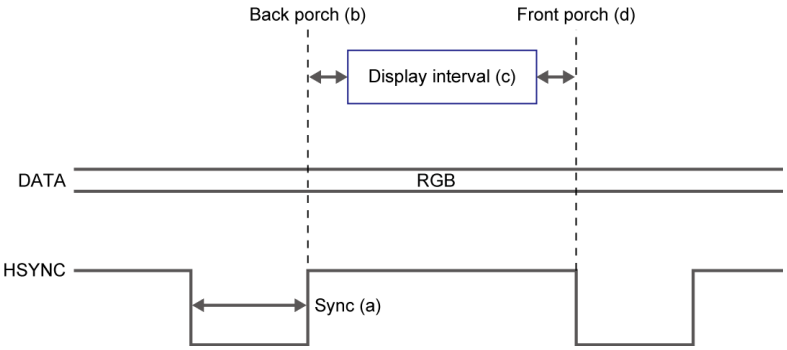
\includegraphics[width=0.5\textwidth]{./images/VGATiming.png}}
	\caption{VGA Timings \cite{terasic_2014}}
\end{figure}
Initially for the IP block the library was created to carry out the VSync and HSync signals which was written by the project group. However, there was a 2ns delay which could not be solved. A number of methods were attempted to correct this 2ns but created a problem with the HSync signal would be 2ns early or 2ns late which was enough to effect the VSync signal that it could not be displayed on a monitor. Due to timing constraints the decision was made to find and implement a pre-made IP and modify it to work on the DE1-SoC board.\cite{stump_2012} The HSync and VSync parts of the IP was used to create the signals. A counter was created to count how many x (Clock signal within display interval) iterations and y (HSync signal) iterations have been completed. The x counter resets on the positive edge of the HSync and the y counter resets on the positive edge of the VSync signal. The IP was then modified to use a full 8 bit colour range available on the DE1-SoC. 
\begin{figure}[H]
	\centering
	\lstinputlisting[language=Verilog, firstline=148, lastline=157, frame=bt]{../VGA_IP.v}
		\caption{X Counter with reset}
\end{figure}
	\begin{figure}[H]
	\centering
	\lstinputlisting[language=Verilog, firstline=286, lastline=292, frame=bt]{../VGA_IP.v}
	\caption{Y Counter with reset}
\end{figure}
The grid was displayed by having an if statement in an always block which checked if x counter or y counter was equal to where a line wanted to be placed. When the counter equalled these values the RGB data signal was set to white. The wave was displayed by passing the x counter through the block to the top layer. This then went to the sampler which had a sample buffer. This data was passed back to the VGA IP which then the value is compared with the y counter. If it is equal to the y counter then the pixel is set to the desired colour. Offsets were added to the waves so it can be controlled 
\end{flushleft}
\newpage
\section{ADC}
\begin{flushleft}
To allow signals to be captured so they can be sampled the onboard analogue-to-digital converter (ADC) was decided to be used. It was decided after having difficulty getting the TerasIC ADDA board to work, so decided to stay within the time constraints to use the onboard ADC. To initialise this QSys was used to generate the appropriate code. The onboard ADC has 4 pins connected to the FPGA. The clock, data in, data out, and CS\_n. QSys allows you to generate the code for these pins in a graphical user interface. It also allows you to select clock speed to update at and the channels you wish to use. The ADC pins allow up to 8 channels of ADC to be used so for expandability all channels where selected to be used. The code was generated and then 2 .v files was copied into the main project and instantiated. The channels where labeled from CH0 to CH7. For this project only CH0 and CH1 were used and the outputs of these were inputted into the sampler. This then samples the values of 800 clock cycles (to match the screen width). This is then ready to be output to the VGA IP.
\begin{figure}[H]
	\centering
	\fbox{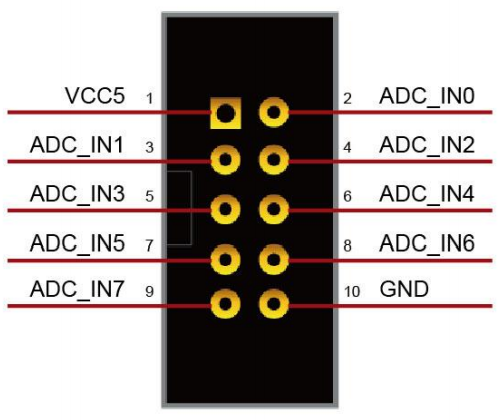
\includegraphics[width=0.5\textwidth]{./images/ADCPins.png}}
	\caption{ADC Pins \cite{terasic_2014}}
\end{figure}

\begin{figure}[H]
	\centering
	\fbox{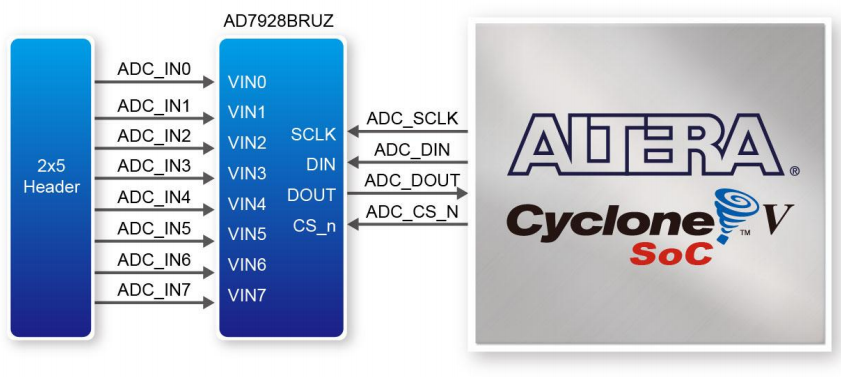
\includegraphics[width=0.5\textwidth]{./images/ADCConnections.png}}
	\caption{ADC Connections to FPGA \cite{terasic_2014}}
\end{figure}
\end{flushleft}
\newpage
\section{Seven Segment Display}
\begin{flushleft}
For measurements to be displayed it was decided for simplicity to use the seven segment display. Each seven segment display is made up of 6 pins which control each part of the seven segments. A limitation was found which did not allow a pin to control the decimal point which was required for our measurements. 
\begin{figure}[H]
	\centering
	\fbox{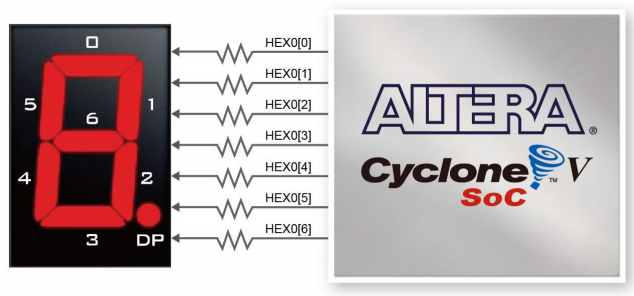
\includegraphics[width=0.5\textwidth]{./images/SevenSeg.png}}
	\caption{Seven Segment Display Pins \cite{terasic_2014}}
\end{figure}
It was very trivial to setup the seven segment display to output a signal number. To do this a register of 7 bits was initialised which could act for each bit of a single seven segment display. It had 2 inputs (clock and number) and then the output for the seven segment display. When a number was entered between 0 to 9 an if statement in an always block was run to give the appropriate output. It was noted that the output is inverted as the seven segment display is active low. 
\begin{figure}[H]
	\centering
	\lstinputlisting[language=Verilog, firstline=138, lastline=167, frame=bt]{../SevenSeg_IP.v}
		\caption{Generate Seven Segment Output Module}
\end{figure}
The next challenge was to have numbers between 0 to 9999 to be separated into singular numbers to be output to the seven segment display. On FPGA division is a very expensive resource. It was decided to use a counter which the idea was taken from online. \cite{stack_overflow} The counter method uses 5 counters, ones, tens, hundreds, thousands, and counter. As the counters count up the ones gets to the number 9 it will reset the ones counter and increase the tens counter. This is the same for the tens, hundreds, and thousands. When the counter reaches the number it then stops and the output number is sent to the seven segment output generator module which turns the numbers into an output for the seven segment displays. This runs at full clock speed so the counting cannot be seen with the human eye. This code can be found on Appendix B.
\end{flushleft}
\newpage
\section{Controls}
\begin{flushleft}
This chapter of the report shall discuss the design of the control IP for the project. The purpose of this module was to enable and control both the cursors, and the waves, such that they appeared on the monitor. They could then be controlled using the keys and the switches, to move, increase/decrease the volts per division, as well as the time per division. This chapter will also discuss the button clock, also known as the slClock. \\ \- \\
Due to the limited number of buttons and switches on the DE1-SoC board, various states were used to decide what was being controlled. These states were controlled by switches 9 and 8. State 1 was the default state when switches 9 and 8 were 0, this state controlled the cursors. State 2 happened when switch 8 was 1 and switch 9 was 0, this state controlled the waves. The final stage was stage 3, and this happened when both switch 9 and 8 were 1, and this displayed the test wave. The purpose of the test wave, was such that while the ADC module was being designed the controls module could still be worked, as well as the VGA module could be tested in hardware. There is a spare state left, which could be used for further expansion in the future. The states and functions shall be described in more detail below. \\ \- \\
The following table below details state 1, when switch 9 and 8 are both 0.  S7 – 0 represents switch 7 to 0, and B3 – 0 represents buttons 3 – 0.\\
\begin{center}
\begin{table}[H]
	\centering
	\begin{tabular}{|c|c|}
	\hline 
	\textbf{Buttons or Switches} & \textbf{Purpose} \\ 
	\hline 
	S7 & N/A \\ 
	\hline 
	S6 & N/A \\ 
	\hline 
	S5 & N/A \\ 
	\hline 
	S4 & N/A \\ 
	\hline 
	S3 & Allow the y-cursors to be moved \\ 
	\hline 
	S2 & Allow the x-cursors to be moved \\ 
	\hline 
	S1 & Enable y-cursors when 1, so that they display on the monitor.
	 \\ 
	\hline 
	S0 & Enable x-cursors when 1, so that they display on the monitor. \\ 
	\hline 
	B3 & \makecell{When S2 is 1 – Move cursor x1 right.\\  When S3 is 1 – Move cursor y1 down.\\ When both S2 and S3 is 1 – Move both x-cursors right.}
	 \\ 
	\hline 
	B2 & \makecell{When S2 is 1 – Move cursor x1 left.\\ When S3 is 1 – Move cursor y1 up.\\ When both S2 and S3 is 1 – Move both x-cursors left.}
	 \\ 
	\hline 
	B1 & \makecell{When S2 is 1 – Move cursor x2 right.\\ When S3 is 1 – Move cursor y2 down.\\ When both S2 and S3 is 1 – Move both y-cursors down.} \\ 
	\hline 
	B0 & \makecell{When S2 is 1 – Move cursor x2 left.\\ When S3 is 1 – Move cursor y2 up.\\ When both S2 and S3 is 1 – Move both y-cursors up.}
	 \\ 
	\hline 
	\end{tabular} 
	\caption{State 1 functions}
\end{table}
\end{center}
\squeezeup
During state 1 if switch 2 and switch 3 are 0, the buttons do nothing. While in state 1 switches 7 to 4 also do nothing. The table below shows state 2, when switch 9 is 0, and switch 8 is 1.\\
\begin{center}
\begin{table}[H]
	\centering
	\begin{tabular}{|c|c|}
	\hline 
	\textbf{Buttons or Switches} & \textbf{Purpose} \\ 
	\hline 
	S7 & N/A \\ 
	\hline 
	S6 & N/A \\ 
	\hline 
	S5 & Adjust the time/division for both waves.  \\ 
	\hline 
	S4 & \makecell{Allows a snapshot in time to be taking of both\\ waves, similar to the run/stop feature on oscilloscopes.}  \\ 
	\hline 
	S3 & Adjust the volts/division for both waves. \\ 
	\hline 
	S2 & Allows both waves to be moved. \\ 
	\hline 
	S1 & Enables wave 2 when 1, so that it displays on the monitor.\\ 
	\hline 
	S0 & Enables wave 1 when 1, so that it displays on the monitor. \\ 
	\hline 
	B3 & \makecell{When S2 is 1 – Move wave 1 down.\\
When S3 is 1 – Increase volts/div for wave 1.\\
When S4 is 1 – Freeze wave 1.\\
When S5 is 1 – Increase time/div for wave 1.}
	 \\ 
	\hline 
	B2 & \makecell{When S2 is 1 – Move wave 1 up.\\
When S3 is 1 – Decrease volts/div for wave 1.\\
When S4 is 1 – Run wave 1.\\
When S5 is 1 – Decrease time/div for wave 1.}
	 \\ 
	\hline 
	B1 & \makecell{When S2 is 1 – Move wave 2 down.\\
When S3 is 1 – Increase volts/div for wave 2.\\
When S4 is 1 – Freeze wave 2.\\
When S5 is 1 – Increase time/div for wave 2.\\
} \\
	\hline 
	B0 & \makecell{When S2 is 1 – Move wave 2 up.\\
When S3 is 1 – Decrease volts/div for wave 2.\\
When S4 is 1 – Run wave 2.\\
When S5 is 1 – Decrease time/div for wave 2.\\
}
	 \\ 
	\hline 
	\end{tabular} 
	\caption{State 2 functions}
\end{table}
\end{center}
\squeezeup
Similar to state 1, the buttons will do nothing if S2 – 5 are all 0. State 3, which occurs when both switch 8 and 9 are 1, enables the test wave to display on the monitor. All cursors and waves move by a size of 1, this is indicated by the localparam moveSize. 
The code for the controls IP can be seen in appendix E. All the controls happen on the positive edge of buttonClock. In appendix A, it can be seen that the buttonClock attaches to the slClock [19]. The code for the slClock can be seen in appendix F. The slClock module was created so that the cursors and waves could be moved accurately. They could not be moved with any precision when running off of the main clock as the main clock ran at 50MHz. This meant that when the cursors or waves moved, they would move to fast to control. However, using the slClock [19] meant that the frequency was approximately 93Hz, and as such was much easier to control.
\end{flushleft}
\newpage
\section{Measurement}
\newpage
\section{Problems Encountered}
\newpage
\section{Conclusion}
\newpage
\section{Appendix}
\subsection{Appendix A - VGA Timing Specifications}
\begin{flushleft}
\begin{table}[H]
	\centering
	\fbox{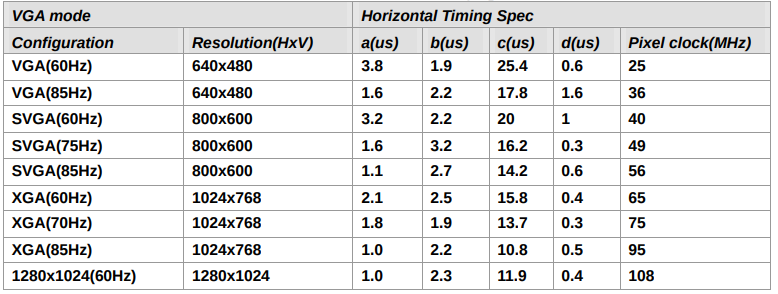
\includegraphics[width=0.9\textwidth]{./images/VGAHTimingSpec.png}}
	\caption{VGA Horizontal Timing Specification \cite{terasic_2014}}
\end{table}
\begin{table}[H]
	\centering
	\fbox{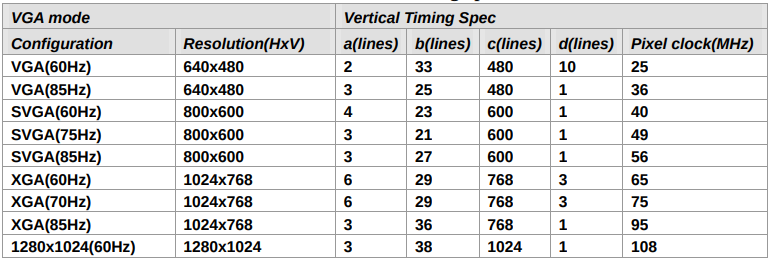
\includegraphics[width=0.9\textwidth]{./images/VGAVTimingSpec.png}}
	\caption{VGA Vertical Timing Specification \cite{terasic_2014}}
\end{table}
\end{flushleft}
\newpage
\addcontentsline{toc}{section}{References}
\begin{flushleft}
\subsection{Appendix B - Number Split Module}
\begin{figure}[H]
	\centering
	\lstinputlisting[language=Verilog, firstline=91, lastline=136, frame=bt]{../SevenSeg_IP.v}
		\caption{Number Split Module}
\end{figure}
\newpage
\bibliography{refs}
\end{flushleft}
\end{document}
